\section{Method}
\label{sec:method}
% ~2 pages incl. Fig. 2 (fig2_method, double column).

\begin{figure*}[t]
  \centering
  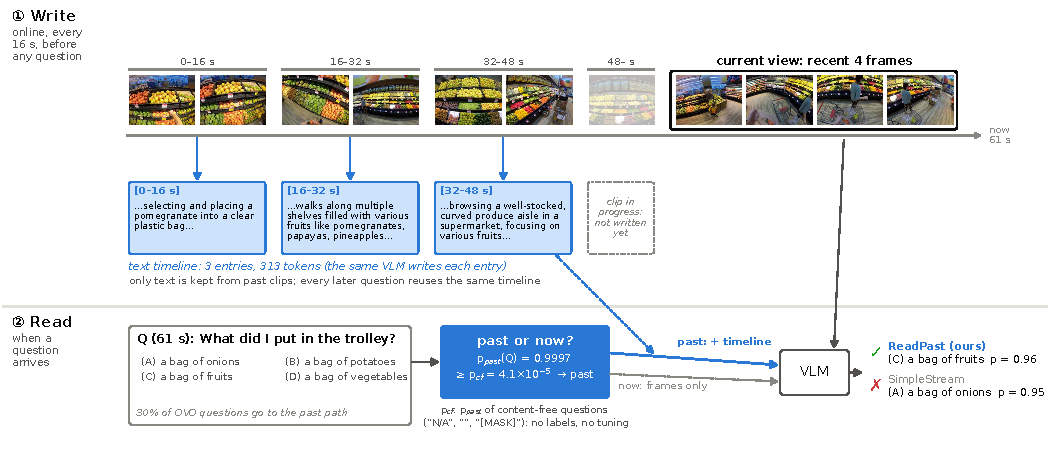
\includegraphics[width=\textwidth]{fig2_method.pdf}
  \caption{Overview of \method{}. \todo{caption}}
  \label{fig:method}
\end{figure*}

\subsection{Problem Setup and the Recent-Window Baseline}
\label{sec:method-setup}
% Stream V, question q at time t with options O. SimpleStream: answer from the last N=4 frames (1 fps sampling).
% Notation for the answer model f, recent frames F_t.
\todo{notation; SimpleStream as $f(F_t, q, O)$.}

\subsection{Self-Written Timeline}
\label{sec:method-timeline}
% Every s=16 s, the same frozen VLM captions 8 frames sampled uniformly in the segment -> (t0, t1, text).
% Timeline M_t = all captions with t1 <= t, prepended before the recent frames (placement ablation: round 10, "before"
% better on 3 backbones). Cost: one 8-frame generation per 16 s of stream; mean 1264 timeline tokens on OVO.
% Writer prompt in appendix.
\todo{writer, schedule, prompt, placement.}

\subsection{Present/Past Gate with Content-Free Calibration}
\label{sec:method-gate}
% Fixed routing prompt on the question text only (no frames, no options: an "Unable to answer" option would leak the task) -> p_past = P("past") / (P("past")+P("now")).
% Threshold p_cf = mean p_past over content-free questions {"N/A", "", "[MASK]"}; read timeline iff p_past >= p_cf.
% One extra forward pass of the text-only prompt per question. Fig. 3 (fig3_calibration): log-odds distributions,
% fixed 0.5 vs p_cf, read rates. Be honest: on LLaVA-OV p_cf is low (RT read rate 40%).
\todo{gate definition, calibration, Fig.~3.}

\subsection{Conditional Abstention Instruction}
\label{sec:method-abstain}
% Instruction text from D-HSM \cite{dhsm}: choose a content option only when evidence supports it, otherwise the
% abstention option. Applied iff O contains an abstention option (e.g., "Unable to answer"); otherwise prompt unchanged.
% Rationale: on questions without such an option the instruction only adds a prior toward refusing / changes answers.
\todo{instruction, trigger rule, rationale.}

\subsection{Cost}
\label{sec:method-cost}
% Write cost amortized per stream second; per-question extra cost = gate forward + timeline prefill. Numbers in
% Sec.~\ref{sec:exp-efficiency}.
\todo{complexity summary.}
